\definecolor{links}{HTML}{2A1B81}
\hypersetup{colorlinks,linkcolor=,urlcolor=links}

\usetheme{Boadilla}
\usecolortheme{seahorse}
\usefonttheme{serif}
\beamertemplatenavigationsymbolsempty

\setbeamertemplate{bibliography item}{\insertbiblabel}

\usepackage{luacode}
\usepackage{luatexja}
\usepackage{pgfpages}
\usepackage[osf]{mathpazo}

\begin{luacode*}
  USE_IPAFONT = os.getenv"USE_IPAFONT"
  USE_YUFONT = os.getenv"USE_YUFONT"
  
  if USE_YUFONT == "true" then
    tex.sprint("\\AtBeginDocument{\\usepackage[yu-osx, deluxe, expert]{luatexja-preset}}")
  elseif USE_IPAFONT == "true" then
    tex.sprint("\\AtBeginDocument{\\usepackage[ipaex, deluxe, expert]{luatexja-preset}}")
  else
    tex.sprint("\\AtBeginDocument{\\usepackage[hiragino-pro, deluxe, expert]{luatexja-preset}}")
  end
\end{luacode*}

\usepackage{epigraph}
\usepackage{etoolbox}
\usepackage{tikz}
\usepackage{framed}
\usepackage{libertine}
\usepackage{amsmath}
\usepackage{mathtools}

\renewcommand{\kanjifamilydefault}{\gtdefault}

%\setbeameroption{show notes on second screen=right}

\setmainfont[Numbers=OldStyle, BoldFont=Palatino Bold]{Palatino}
\setsansfont{CMU Sans Serif}
\setmonofont{CMU Typewriter Text}

\input{vc.tex}

\title[\href{http://qiita.com/yyu/items/fce9b33c784e0631ddf6}{公平なガチャシステム}]{%
  \href{http://qiita.com/yyu/items/fce9b33c784e0631ddf6}{公平なガチャシステム}
}
\author{吉村 優}
\date[July 25, 2016]{%
  July 25, 2016 \\%
  {\footnotesize (Commit ID: \GITAbrHash)}
}
\institute[\href{https://twitter.com/\_yyu\_}{@\_yyu\_}]{%
  \url{https://twitter.com/\_yyu\_}\\
  \url{http://qiita.com/yyu}\\
  \url{https://github.com/y-yu}\\
}

\newfontfamily\quotefont[Ligatures=TeX]{Linux Libertine O} % selects Libertine as the quote font

\newcommand*\quotesize{60} % if quote size changes, need a way to make shifts relative
% Make commands for the quotes
\newcommand*{\openquote}
   {\tikz[remember picture,overlay,xshift=-4ex,yshift=-2.5ex]
   \node (OQ) {\quotefont\fontsize{\quotesize}{\quotesize}\selectfont``};\kern0pt}

\newcommand*{\closequote}[1]
  {\tikz[remember picture,overlay,xshift=1.5ex,yshift={#1}]
   \node (CQ) {\quotefont\fontsize{\quotesize}{\quotesize}\selectfont''};}

\newcommand*\shadedauthorformat{\emph} % define format for the author argument

% Now a command to allow left, right and centre alignment of the author
\newcommand*\authoralign[1]{%
  \if#1l
    \def\authorfill{}\def\quotefill{\hfill}
  \else
    \if#1r
      \def\authorfill{\hfill}\def\quotefill{}
    \else
      \if#1c
        \gdef\authorfill{\hfill}\def\quotefill{\hfill}
      \else\typeout{Invalid option}
      \fi
    \fi
  \fi}
% wrap everything in its own environment which takes one argument (author) and one optional argument
% specifying the alignment [l, r or c]
%
\newenvironment{shadequote}[2][l]%
{\authoralign{#1}
\ifblank{#2}
   {\def\shadequoteauthor{}\def\yshift{-2ex}\def\quotefill{\hfill}}
   {\def\shadequoteauthor{\par\authorfill\shadedauthorformat{#2}}\def\yshift{2ex}}
\begin{quote}\openquote}
{\shadequoteauthor\quotefill\closequote{\yshift}\end{quote}}

\makeatletter
\def\@fnsymbol#1{\ensuremath{\ifcase#1\or *\or \dagger\or \ddagger\or
   \mathsection\or \mathparagraph\or \|\or **\or \dagger\dagger
   \or \ddagger\ddagger \else\@ctrerr\fi}}
\makeatother

\renewcommand{\thefootnote}{\fnsymbol{footnote}}

\usetikzlibrary{shapes.callouts} 

\pgfkeys{%
    /calloutquote/.cd,
    width/.code                   =  {\def\calloutquotewidth{#1}},
    position/.code                =  {\def\calloutquotepos{#1}}, 
    author/.code                  =  {\def\calloutquoteauthor{#1}},
    /calloutquote/.unknown/.code   =  {\let\searchname=\pgfkeyscurrentname
                                 \pgfkeysalso{\searchname/.try=#1,                                
    /tikz/\searchname/.retry=#1},\pgfkeysalso{\searchname/.try=#1,
                                  /pgf/\searchname/.retry=#1}}
                            }  


\newcommand\calloutquote[2][]{%
       \pgfkeys{/calloutquote/.cd,
         width               = 5cm,
         position            = {(0,-1)},
         author              = {}}
  \pgfqkeys{/calloutquote}{#1}                   
  \node [rectangle callout,callout relative pointer={\calloutquotepos},text width=\calloutquotewidth,/calloutquote/.cd,
     #1] (tmpcall) at (0,0) {\hfil#2\hfil};
  \node at (tmpcall.pointer){\calloutquoteauthor};    
}


\newcommand\ballref[1]{%
\tikz \node[circle, shade,ball color=structure.fg,inner sep=0pt,%
  text width=8pt,font=\tiny,align=center] {\color{white}\ref{#1}};
}

\begin{document}

\frame{\maketitle}

\section{自己紹介}
\begin{frame}
  \frametitle{自己紹介}
  
  \begin{columns}
    \begin{column}{0.3\textwidth}
      \centering
      \begin{figure}
        
\includegraphics[width=0.95\textwidth]{img/bird2x.png}
      \end{figure}
    \end{column}
    \begin{column}{0.7\textwidth}
      \begin{itemize}
        \item<2-> 筑波大学 情報科学類卒(学士)
      \end{itemize}
    \end{column}
  \end{columns}
\end{frame}

\section{ガチャとは?}

\begin{frame}
  \frametitle{ガチャとは?}

  \begin{itemize}
    \item<2-> ソーシャルゲームなどに実装された機能のひとつ
    \item<3-> お金を投入すると\textbf{確率}で特定のカードを入手できる
  \end{itemize}

  \begin{center}
    \uncover<4->{
      \begin{tikzpicture}
        \calloutquote[width=5cm,position={(0.7,-0.2)},fill=blue!30,rounded corners]{誰が確率を計算するの?}
      \end{tikzpicture}
    }

    \uncover<5->{
      \begin{tikzpicture}
        \calloutquote[width=4cm,position={(-0.5,-0.2)},fill=green!30,rounded corners]{運営のサーバー?}
      \end{tikzpicture}
    }

    \uncover<6->{
      \begin{tikzpicture}
        \calloutquote[width=9cm,position={(0.9,-0.2)},fill=red!30,rounded corners]{サーバーの実装が正しい確率に従っているのか?}
      \end{tikzpicture}
    }
  \end{center}
\end{frame}

\begin{frame}
  \frametitle{ガチャの確率に対する疑惑}

  \begin{center}
    \uncover<2->{
      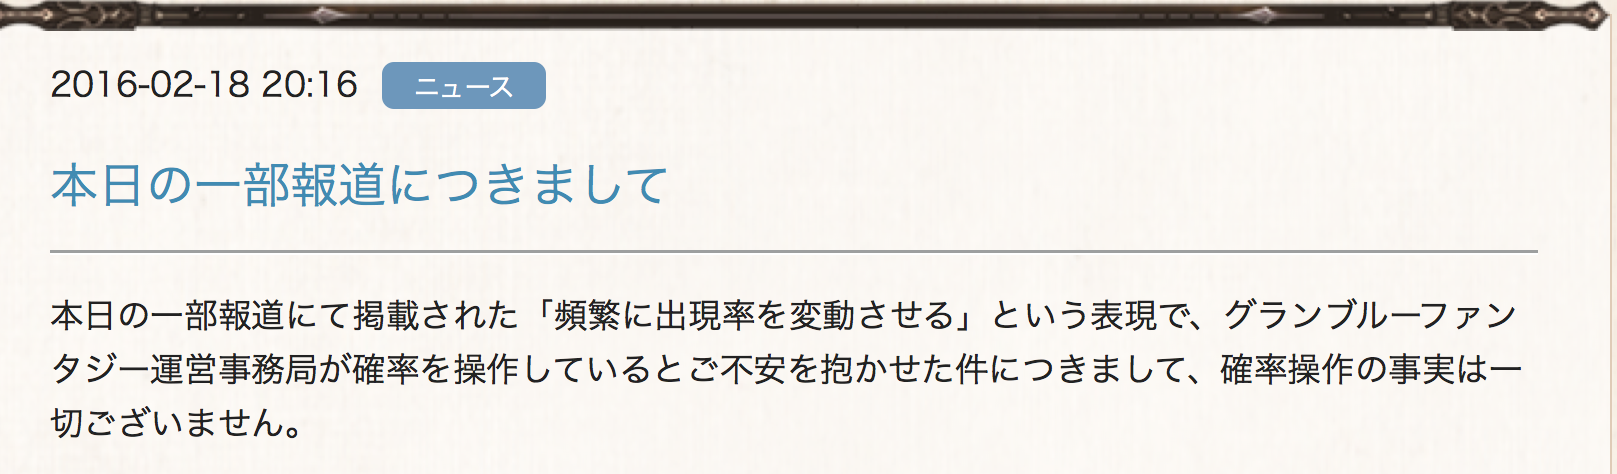
\includegraphics[width=0.9\textwidth]{img/grablu.png}
    }
  \end{center}

  \uncover<3->{
    サーバーで計算される確率に対して疑惑を抱いている人もいる
  }

  \begin{center}
    \uncover<4->{
      \begin{tikzpicture}
        \calloutquote[width=9cm,position={(-0.7,-0.2)},fill=green!30,rounded corners]{サーバーで計算される確率を検証するのは無理}
      \end{tikzpicture}
    }

    \uncover<5->{
      \begin{tikzpicture}
        \calloutquote[width=7cm,position={(0.7,-0.2)},fill=blue!30,rounded corners]{クライアントサイドで計算すれば?}
      \end{tikzpicture}
    }

    \uncover<6->{
      \begin{tikzpicture}
        \calloutquote[width=7cm,position={(-0.7,-0.2)},fill=red!30,rounded corners]{リバースエンジニアリングの餌食!}
      \end{tikzpicture}
    }
  \end{center}
\end{frame}

\section{公平なガチャシステム}
\begin{frame}
  \frametitle{公平なガチャシステム}

  次のような\textbf{公平なガチャシステム}が欲しい
  \begin{itemize}
    \item<2-> ユーザーにとっても運営にとってもガチャによるカードの出現確率が実装に基づいて明らかである
    \item<3-> 悪意を持つユーザーや悪意を持つ運営による確率操作ができない
  \end{itemize}

  \uncover<4->{
    \begin{block}{従来の公平なガチャ}
      \begin{itemize}
        \item<5-> ハッシュ値の衝突に基づくガチャ\cite{hash}
        \item<6-> 対称鍵暗号に基づくガチャ\cite{mala}
      \end{itemize}
    \end{block}
  }

  \begin{center}
    \uncover<7->{
      \begin{tikzpicture}
        \calloutquote[width=6cm,position={(0.7,-0.2)},fill=blue!30,rounded corners]{これらを使えばいいのでは?}
      \end{tikzpicture}
    }

    \uncover<8->{
      \begin{tikzpicture}
        \calloutquote[width=3cm,position={(-0.5,-0.2)},fill=red!30,rounded corners]{課題がある!}
      \end{tikzpicture}
    }
  \end{center}
\end{frame}

\begin{frame}
  \frametitle{ハッシュ値の衝突に基づくガチャ\cite{hash}}

  \begin{enumerate}
    \item<2-> サーバーはユーザーにソルト$A$とデータ$C$を送信する
    \item<3-> ユーザーは次を満たすデータ$B$を探索する\footnote[frame]{$\&$は論理積を意味し、$\mid\mid$は文字列の結合を意味する}
      \[
        M(K_i) = C\, \&\, \text{Hash}(A \mid\mid B)
      \]
    \item<4-> ユーザーはデータ$B$をサーバーへ送信する
    \item<5-> サーバーはデータを検証し、正しければカード$K_i$を授与する
  \end{enumerate}

  \uncover<6->{
    \begin{alertblock}{課題}
      \begin{itemize}
        \item<7-> 時間あたりに計算できるハッシュ値の数が、そのままガチャを試行できる回数になる
        \item<8-> 専用ハードウェアを持つ業者など、ハッシュ値の計算能力が高い人が有利である
      \end{itemize}
    \end{alertblock}
  }
\end{frame}

\begin{frame}
  \frametitle{対称鍵暗号に基づくガチャ\cite{mala}}

  \begin{enumerate}
    \item<2-> 
      \label{enum:encryption}
      サーバーは値$m$を対称鍵で暗号化して、その暗号文$c$をユーザーへ送信する
    \item<3-> ユーザーは任意のカード$x$を選択しサーバーへ送信する
    \item<4->
      \label{enum:opening}
      サーバーは$c$の対称鍵をユーザーへ公開する
    \item<5-> ユーザーは次のカード$k$を入手する\footnote[frame]{$N$はカードの種類の数である}
      \[
        k := (x + m) \bmod N
      \]
  \end{enumerate}

  \uncover<6->{
    \begin{alertblock}{課題}
      \begin{itemize}
        \item<7-> サーバーは\ballref{enum:encryption}で用いた鍵と、
          \ballref{enum:opening}で公開する鍵を別にしたとしても、ユーザーはそれを検証できない
        \item<8-> サーバーはカードを操作できるので、サーバーが有利である
      \end{itemize}
    \end{alertblock}
  }
\end{frame}

\begin{frame}
  \frametitle{対称鍵暗号に基づくガチャ\cite{mala}}

  \begin{center}
    \begin{tikzpicture}
      \calloutquote[width=9cm,position={(0.7,-0.3)},fill=green!30,rounded corners]{対称鍵暗号では、暗号化に使う鍵と復号に使う鍵が同じと保証できない}
    \end{tikzpicture}

    \uncover<2->{
      \begin{tikzpicture}
        \calloutquote[width=10cm,position={(-0.7,-0.3)},fill=cyan!30,rounded corners]{やりたいのは情報を与えずに、後からの変更を防ぐこと}
      \end{tikzpicture}
    }

    \uncover<3->{
      \begin{tikzpicture}
        \calloutquote[width=5cm,position={(0.7,-0.3)},fill=red!30,rounded corners]{\textbf{コミットメント}を使う!}
      \end{tikzpicture}
    }
  \end{center}
\end{frame}

\section{コミットメント}

\begin{frame}
  \frametitle{コミットメント\cite{Hans_Helmut_林200312}}

  \uncover<2->{
    \begin{block}{コミットメント}
      \begin{description}
        \item[コミット] 送信者はコミットしたい情報$b$を暗号化して受信者に送信する
        \item[公開] 送信者は受信者が$b$を復元できるように付加的な情報を受信者に送信する 
      \end{description}
    \end{block}
  }

  \begin{itemize}
    \item<3-> コミットのステップでは、受信者はコミットされた値について何も分からない
    \item<4-> 送信者はコミットのステップ後に、コミットした値を変更することができない
  \end{itemize}
\end{frame}

\section{コミットメントを導入したガチャシステム}

\begin{frame}[label=protocol]
  \frametitle{コミットメントを導入したガチャシステム\cite{commitment}}

  \begin{enumerate}
    \item<2-> ユーザーは$p = 2q + 1$となる大きな素数$p, q$をランダムに生成して、
      $\mathbb{Z}^*_p$\footnote[frame]{整数$x = y \bmod p$かつ$xz \equiv 1 \pmod{p}$となる$y$と逆元$z$が存在する$x$の集合である}
      の位数$q$の部分群$G$から\textbf{生成元}$g, v \ne 1$をランダムに選択して$p, q, g, v$をサーバーへ送信する
    \item<3-> サーバーは$p, q, g, v$を検証し、ランダムに$m \in \{1, \dots, q - 1\}$を選択し、
      乱数$r \in \{1, \dots, q - 1\}$を用いて$c := g^r v^m \bmod p$計算し$c$をユーザーへ送信する
    \item<4-> ユーザーはランダムにカードの番号$x$を選び、サーバーへ送信する
    \item<5-> サーバーは$r, m$を公開する
    \item<6-> ユーザーは$c \equiv g^r v^m \pmod{p}$を検証し、次の番号$k$に対応するカードを得る
      \[
        k := (m + x) \bmod N
      \]
  \end{enumerate}
\end{frame}

\begin{frame}[fragile, label=mdash]
  \frametitle{コミットメントの検証}
  
  \begin{center}
    \uncover<2->{
      \begin{tikzpicture}
        \calloutquote[width=7cm,position={(-0.7,-0.3)},fill=green!30,rounded corners]{サーバーが$m$を後から変更する?}
      \end{tikzpicture}
    }

    \uncover<3->{
      サーバーは$m$をコミットした後で、$m'(m' \ne m)$と偽れる

      {\Large$\Downarrow$\scriptsize ならば}
    }

    \uncover<4->{
      サーバーは$g^r v^m = g^{r'} v^{m'}$となる$r'$を計算できる

      {\Large$\Downarrow$\scriptsize ならば}
    }

    \uncover<5->{
      サーバーは$g$を何乗したら$v$となるかという\textbf{離散対数}が求められる

      \begin{align*}
        g^r v^m    &= g^{r'} v^{m'}      \\
        v^{m - m'} &= g^{r' - r}         \\
        \log_g{(v^{m - m'})} &= r' - r   \\
        \log_g{(v)} &= (r' - r) / (m - m') 
      \end{align*}
    }
  \end{center}
\end{frame}

\begin{frame}
  \frametitle{離散対数問題\cite{光成201506}}

  \uncover<2->{
    \begin{exampleblock}{定義}
      $g, p, g^x \bmod p$が与えられたとき、$x$を求める問題のことである
    \end{exampleblock}
  }

  \uncover<3->{
    \begin{block}{}
      $g, p$が次を満すとき、離散対数問題を現実的な時間内に解くことは困難である
      \begin{itemize}
        \item<4-> $p$は1024ビット以上の素数
        \item<5-> $p - 1$の約数の中に、$p$に近いサイズの素数$q$が含まれている
        \item<6-> $g$が生成元\footnote[frame]{%
            生成元は全ての$i = 1, \dots, q - 1$と$j = 1, \dots, q - 1$について、
            $i \ne j$ならば$g^i \not\equiv g^j \pmod{p}$となる}である
      \end{itemize}
    \end{block}
  }
\end{frame}

\begin{frame}
  \frametitle{コミットメントの検証}

  \begin{center}
    サーバーは$m$をコミットした後で、$m'(m' \ne m)$と偽れる

    {\Large$\Downarrow$\scriptsize ならば}

    サーバーは$g$を何乗したら$v$となるかという\textbf{離散対数}が求められる
  \end{center}

  \uncover<2->{
    \begin{alertblock}{}
      \begin{center}
        離散対数問題を解くことは困難であるということに矛盾する
      \end{center}
    \end{alertblock}
  }

  \uncover<3->{
    \begin{block}{}
      \begin{center}
        サーバーが$m$をコミットした後で$m'$と変更することは困難である
      \end{center}
    \end{block}
  }
\end{frame}

\section{まとめ}
\begin{frame}
  \frametitle{まとめ}
  
  \begin{itemize}
    \item<2-> ガチャシステムにおけるサーバーサイドの確率計算に疑念を抱くユーザーがいる
    \item<3-> 従来の公平なガチャには微妙に公平ではない部分がある
    \item<4-> 今回提案したガチャは、コミットメントを用いて完全な公正性を目指した
  \end{itemize}
\end{frame}

\section*{参考文献}
\begin{frame}
  \frametitle{参考文献}

  \bibliographystyle{junsrt_url}
  \nocite{*}
  \bibliography{ref}
\end{frame}

\begin{frame}
  \frametitle{目次}

  \tableofcontents[hideallsubsections]
\end{frame}

\begin{frame}
  \centering
  {\Huge Thank you for listening!}

  \quad \quad

  {\Huge Any question?}
\end{frame}

\end{document}
